%!TEX encoding = UTF-8

\chapter{Affordances and Planning}
\label{chap:poeticon++_case_study}

This chapter presents a case study of the application of the ideas presented in the previous chapters~(namely affordances, language, and tool use) within the scope of the European research project POETICON++.
See Fig.~\ref{fig:poeticon++_logo_and_description} for a brief description of that project.

We show how robot sensorimotor knowledge (learned affordances) can be combined with symbolic reasoning, forming a unified \emph{planning architecture}.
We use probabilistic reasoning to permit a robot to carry out a complex manipulation task, requested by a human user with verbal language, under challenging conditions and external disturbances.

\begin{figure}
\centering
\includegraphics[width=0.4\textwidth]{logopoeticonplusplus150dpi-ebook} % white bg
\caption[Logo of the POETICON++ project.]{Logo of the POETICON++ project \allowbreak (\url{http://www.poeticon.eu/}).
The main objective of this project was to develop computational models and machinery for robots that would allow them to generalize motor execution and visual experiences beyond the ones known at learning time, resorting to natural language reasoning.}
\label{fig:poeticon++_logo_and_description}
\end{figure}

This chapter is the subject of the following publications:
\listPublicationsPoeticonpp

The rest of this chapter is structured as follows.
Sec.~\ref{sec:poeticon++:motivation} gives the background and motivation for the case study.
Sec.~\ref{sec:poeticon++:related_work} overviews the literature of robot reasoning architectures similar to ours.
Sec.~\ref{sec:poeticon++:setup} states our main objective, assumptions and approach.
Sec.~\ref{sec:poeticon++:proposed_approach} illustrates our proposed architecture and its constituent parts.
We report experimental robot results in Sec.~\ref{sec:poeticon++:results}.
Finally, in Sec.~\ref{sec:poeticon++:conclusions} we give our concluding remarks.

\section{Motivation}
\label{sec:poeticon++:motivation}

\begin{figure}
\centering
\includegraphics[trim=0.5cm 0cm 0cm 1.5cm,clip, width=0.9\linewidth]{icub_with_objects-low_viewpoint_1}
\caption[A robot performing a complex manipulation task after receiving a verbal instruction from a human.]{A robot performing a complex manipulation task after receiving a verbal instruction from a human.
In the back screen, images from the robot cameras showing visual perception routines.}
\label{fig:icub_with_objects}
\end{figure}

As robots are increasingly moving to unstructured settings (e.g., homes and public places, see~\cite{prassler:2016:domestic}), they must be able to carry out \emph{complex manipulation tasks} alongside humans, also in the presence of \emph{uncertainty}.
Indeed, the shift from industrial to service robots bears the issue of how to design artificial agents that can work effectively with humans performing manual tasks, in a scenario like the one of Fig.~\ref{fig:icub_with_objects}: a human verbally instructing a robot to perform a manipulation task.
In particular, major challenges faced by the robot in such a situation are:
(i)~how to understand and execute instructions provided by human users (see Fig.~\ref{fig:sandwich_xkcd}), taking into consideration the properties of the available objects and the uncertainty in robot action and perception;
(ii)~how to monitor and adapt to an unstructured~(non-industrial) environment which will be constantly evolving and changing during task execution~\cite{haazebroek:2011:cognprocess}.

\begin{figure}
\centering
\includegraphics[width=0.6\textwidth]{sandwich-xkcd149}
% footnote within caption, https://tex.stackexchange.com/a/67030
\caption[A comic strip about the subtleties of asking another agent to prepare a sandwich.]{A comic strip about the subtleties of asking another agent to prepare a sandwich. Reproduced under the CC BY-NC~2.5 license from~\url{https://xkcd.com/149/}\protect\footnotemark.\ In the POETICON++ project, the final demonstration also consisted of asking a robot to make a sandwich, using the available tools and ingredients present in the scene, as explained in this chapter.}
\label{fig:sandwich_xkcd}
\end{figure}
\footnotetext{Explanation of the comic strip of Fig.~\ref{fig:sandwich_xkcd}: on UNIX and Linux computer systems, users can be assigned to all kinds of rights, for example rights to access to certain directories and to execute certain commands. The \emph{sudo} command lets certain authorized users override these policies by executing the command (everything after the word \emph{sudo} on the command line) as the administrator root user. Forgetting to start the command with \emph{sudo} is a fairly common and frustrating mistake for people who administer UNIX-like systems. They then need to repeat the command with \emph{sudo}, at which point the computer responds obediently, and everything works smoothly.}

Bearing these challenges in mind, in this chapter we present a robot action selection system that combines
(i)~robot sensorimotor knowledge~(in the form of learned affordances) with
(ii)~symbolic reasoning, by resorting to a unified probabilistic representation; moreover, this system is seamlessly integrated in a bigger control architecture which includes
(iii)~formulation of robot goals from human verbal requests,
(iv)~continuous perception of the world through robot sensing,
(v)~execution monitoring and re-planning with heuristics.

This chapter contains:
a thorough description of our framework from the systems perspective, including the strategies~(e.g., heuristics) devised for applying our system profitably;
qualitative tests of our architecture on a real humanoid robot;
a quantitative evaluation of the architecture, simulating the execution of a human-specified instruction under varying levels of uncertainty and with different planning strategies and heuristics.

We have implemented our architecture on the iCub humanoid robot (see Sec.~\ref{sec:platform:icub}), validating our system, showing how the overall architecture allows complex robotic problem solving of manual tasks specified by humans, coping efficiently with different levels of uncertainty.
We publicly release our code\footnote{\url{https://github.com/robotology/poeticon} \label{footnote:poeticon_repo}}, including a simulated symbolic reasoner for validating the probabilistic planner under challenging conditions, and real robot sensorimotor data used for affordance learning.
The public repository contains additional material, e.g., a video of the system implemented on the iCub.

\section{Related Work}
\label{sec:poeticon++:related_work}

In this case study we consider a \emph{cognitive architecture} that allows a humanoid robot to understand generic instructions provided in natural language~(i.e., \emph{\acl{NLU}} or \acs{NLU}), and to execute them by combining \emph{affordance perception} and \emph{action planning}: below, we report relevant previous works in these areas.

%%%%%%%%%%%%%%%%%%%%%%%%%%%%%%%%%%%%%%%%%%%%%%%%%%%%%%%%%%%%%%%%%%%%%%%%%%%%%%%%
\subsection{Cognitive Architectures}

In \ac{AI} and robotics literature, several comprehensive cognitive architectures for making robots accomplish complex tasks have been proposed~\cite{vernon:2016:bica}.
Given their interdisciplinary scope, these architectures are typically modular.
They contain multiple components which address the specific requirements~(e.g., \acs{NLU}, planning under uncertainty, probabilistic inference, sensor fusion, execution monitoring, robot manipulation), although there is no single framework that is suited for all applications, given their great diversity~\cite{beetz:2016:ai-reasoning}.
Examples of comprehensive cognitive architectures for robots are~\cite{py:2010:aamas,haazebroek:2011:cognprocess,sisbot:2012:tro,lemaignan:2017:ai,moulin-frier:2018:tcds}.
While these systems present solid theoretical foundations in behavior-based control and robot simulation results, they do not focus on robustness to uncertainty and noise, on re-planning, or on the applicability to general scenarios~(i.e., not being restricted to one specific task) on real robot platforms such as humanoids equipped with many degrees of freedom.
An interesting work is~\cite{ramirez-amaro:2015:ai}, which shows a reasoning system for transferring goal-oriented skills by imitation between two agents, human and robot.
This system gives an iCub humanoid robot the ability to recognize the action performed by a human demonstrator, to extract semantic properties from that action, and to replicate the goal of that action autonomously at a later moment.
Our work has analogies with it, given that we also introduce a goal reasoning and execution system deployed on the iCub robot, however
(i)~we consider actions expressed in natural language, being then grounded and translated to a~(potentially long) sequence of sub-goals for autonomous robot planning and execution;
(ii)~we focus on the unified probabilistic integration of robot affordances with probabilistic planning, which together provide our system some leeway to recover from unexpected events and failures, as well as generalization ability when presented with novel objects not seen in the training phase.

In~\cite{caccavale:2017:icdl}, a framework for imitation learning of sequential tasks is proposed, using human demonstrations to have a robot execute a pizza topping task.
That work is focused on learning movement primitives without supervision in dual-arm assembly settings, assuming for simplicity that the downmost ingredient of the structure to assemble~(i.e., the pizza dough) is known \apriori{} and that it is located within an area reachable by both robot arms; additionally, there is no explicit fault detection mechanism to monitor task execution and to react to failures.
By contrast, our work addresses arbitrary locations of the objects to be used by the robot~(including ones that are not reachable with bare robot hands but might become reachable when resorting to tools).
In addition we explicitly incorporate mechanisms and heuristics for re-planning and recovery from failure, as mentioned above.

In~\cite{moulin-frier:2018:tcds}, an architecture for complex collaborative tasks between a human and an iCub humanoid robot is proposed, integrating different robot skills such as perception, manipulation, and social interaction capabilities with a speech interface and generation of verbal descriptions of events.
That work has similarities with our proposed approach, being targeted to a \hr{} collaboration task using language.
However, the authors employ planning at a local level, meaning that they envision a list of successive actions requested explicitly by a human user to a robot, one after another~(i.e., ``take the cube'', ``point to the octopus toy''), and then, for each action, a sequence of sub-actions with pre-conditions and post-conditions is considered, selecting and executing the one with the shortest length.
Each motor action is repeated~(up to a pre-defined timeout) until the post-conditions are met, and visual-linguistic knowledge is incorporated to guide action selection.
By contrast,
(i)~we use probabilistic planning at a global level, going from a single human instruction in natural language~(i.e., the final goal) to an entire plan that instantiates a list of sub-goals and robot motor actions, reasoning on their probabilities of success, which are updated during task execution and monitoring;
(ii)~when an object is needed but it is not reachable by the robot, we use tool affordance knowledge to have the robot select the best tool in order to bring the object closer autonomously and carry on with the greater plan, whereas in~\cite{moulin-frier:2018:tcds} the robot asks the help of the human partner to position the object closer to the robot;
(iii)~to address failures of individual actions, we use probabilistic strategies and heuristics~(e.g., the robot tries to use an alternative arm or an alternative ingredient if the first one has failed repeatedly) instead of pre-defined timeouts.

%%%%%%%%%%%%%%%%%%%%%%%%%%%%%%%%%%%%%%%%%%%%%%%%%%%%%%%%%%%%%%%%%%%%%%%%%%%%%%%%
\subsection{\acl{NLU}}
\label{sec:poeticon++:related_work:nlu}

The work by Tellex~\cite{tellex:2011:aaai,tellex:2011:ai} is geared at interpreting language commands given to mobile robots with statistical symbol grounding, i.e., mapping words to syntactic structures of concrete objects, paths and events~\cite{harnad:1990}, possibly with unsupervised learning \cite{taniguchi:2016:advr}.
Along with grounding, many works also handle symbol anchoring~\cite{coradeschi:2003:ras,lemaignan:2012:ijsr,elfring:2013:ras}.
Anchoring refers to the process of linking language symbols to real-world representations acquired with robot sensing: it requires appropriate strategies when the process takes place over time in a dynamic environment.
We implement the anchoring aspect in our world modeling component~(see Sec.~\ref{sec:poeticon++:proposed_approach:worldstate}).
In \cite{matuszek:2012:icml,matuszek:2013:er}, language and perception signals are learned jointly by a robot, which is then able to disambiguate generic instructions (e.g., ``go'') using contextual cues; however, no error recovery mechanism is present.
Similarly, in~\cite{chen_mooney:2011:aaai} a semantic parser is learned by observing a human instructor perform a set of motor actions related to navigation, also without recovery from failure.

When it comes to available \emph{general} knowledge bases of natural language applicable to robotics~(in the sense that they are not just geared towards a specific problem like understanding navigation instructions, but span multiple domains), \emph{semantic reasoning} engines for translating human language into robot instructions have been proposed, for instance PRAXICON~\cite{pastra:2008:praxicon,mavroeidis:2016:praxicon} and DIARC~\cite{dzifcak:2009:icra}. DIARC is an architecture for translating natural language instructions and executing them on a robot.
However, while that system has a failure detection mechanism, it does not re-plan, nor does it use prior robot action knowledge to generalize to unseen objects and tools as done in the present work.
In~\cite{misra:2016:ijrr}, a statistical method for grounding natural language instructions to specific robot environments in kitchen and home scenarios is proposed, being able to handle missing and incomplete instructions in the human language input, such as in ``heat up the water, then cook the ramen''~(inferring how to cook the object in this scenario).
Similarly, the framework of~\cite{eppe:2016:iros} analyzes specific language understanding problems and ambiguities that frequently arise in \hri.
In PRAXICON, which we adopt in our architecture, a human instruction is decomposed into a set of deterministic human-like actions such as ``hand grasps knife, knife cuts tomato, \dots''.
However, this type of sequence does not take into account the geometric world around the robot, thus requiring planning over each instruction for a physical implementation.

%%%%%%%%%%%%%%%%%%%%%%%%%%%%%%%%%%%%%%%%%%%%%%%%%%%%%%%%%%%%%%%%%%%%%%%%%%%%%%%%
\subsection{Affordance Perception and Planning}

Affordances are useful in robotics because they model essential properties of environment objects in terms of the actions that a robot is able to perform with them (see Ch.~\ref{chap:motivation} and~\ref{chap:background}).
We now cite a few works that link affordances with action planning, being relevant for this chapter.

In~\cite{moldovan:2018:ar} the relational affordances between objects pairs are exploited to plan a sequence of actions to achieve a desired goal, using probabilistic reasoning; however, how these interactions are affected by different geometrical properties of the objects is not investigated.
Some authors have suggested an alternative computational model called \emph{\acfp{OAC}} \cite{kruger:2011:ras}, which links low-level sensorimotor knowledge with high-level symbolic reasoning hierarchically in autonomous robots, similarly to how we will use affordances for planning in this chapter.
However, the practical uses reported up to the time of writing this thesis correspond to simple examples, pre-defined transition rules and high-level relations, excluding typical problems that characterize real-world robot behaviors: noise, errors in perception, execution failure, unexpected events.
By contrast, the literature on robot affordances reports results from real (i.e., not simulated) robot experiments that tackle those problems explicitly.

In~\cite{ugur:2015:icra} a robot first learns affordance categories and then high-level logical rules, which are encoded in \ac{PDDL}, enabling symbolic planning with off-the-shelf \ac{AI} planners.
In a follow-up work~\cite{ugur:2015:humanoids} the generated plans are used in a real-world object stacking task and new affordances that appear during plan execution are discovered.
The robot is able to build stable towers exhibiting interesting reasoning capabilities, such as stacking larger objects before smaller ones, and the ability to generalize by object types~(assuming that the robot is able to visually detect objects, to extract their features before learning, and that object relations such as relative differences in diameter have been previously learned in simulation).

The system of~\cite{ugur:2015:icra,ugur:2015:humanoids} focuses on learning a parameterized symbolic representation from robot manipulation experiments, and is useful for planning probabilistically with unknown objects.
Our system focuses on combining affordance perception with probabilistic planning, too, but we include tool use affordance capabilities~(to overcome the geometric difficulties of objects being far away from the robot), as well as heuristic strategies for recovering from failures and re-planning, thus providing a system that is robust under manipulation noise.
Furthermore, the tools that our system is able to use do not need to be previously learned by object recognition.

Task and motion \emph{planning} have been combined together in several \ac{AI} and robotic works~\cite{lozano:1987:icra,srivastava:2014:icra}.
Hierarchical planning~\cite{nourbakhsh:1998:wac} has provided algorithms like SHOPS2~\cite{goldman:2009:icaps,wolfe:2010:icaps}.
These methods combine symbolic and geometrical planning, however they usually employ one static plan to be followed and completed by the agent, not allowing failures or re-planning.
Further work exists on simultaneous plan and execution~(\acl{HPN} or \acs{HPN}~\cite{pasula:2007:jair,kaelbling:2011:icra}), focused specifically on the execution of geometrical problems, merging symbols with geometric planning.
The problem of real-time planning and execution requires an algorithm that can adapt to changes in the state.
\acs{HPN} introduces this by updating a world state model at each step, and planning from there.
By using a hierarchy of actions, it transforms a hard problem into several smaller ones that are more easily solved by a planner.
This approach was initially suggested by Nourbakhsh~\cite{nourbakhsh:1998:wac}, where a big problem would be turned into smaller ones by completing sub-goals and re-planning.

\begin{figure*}
\centering
\includegraphics[width=0.9\textwidth]{diagram_for_poeticon++_thesis_chapter}
\caption[POETICON++ architecture exposing the main components of our system.]{POETICON++ architecture exposing the main components of our system.
In the bottom left, a human user expresses an instruction in natural language.
In the bottom right, a robot reasons about the environment and executes the instruction.
The robot can be real or simulated.
The components~(software modules) of the system are represented as gray rectangles, or gray cylinders in case they incorporate a knowledge base.
Arrows indicate data flow.}
\label{fig:poeticon++_diagram}
\end{figure*}

Multi-level planning based on~\cite{nourbakhsh:1998:wac} has been explored in~\cite{wolfe:2010:icaps,kaelbling:2011:icra,lozano:2014:iros}, using a set of pre-determined robot instructions.
By contrast, our approach creates a full chain, from a very abstract human instruction to specific motions at the lower control level, as shown in Fig.~\ref{fig:poeticon++_diagram}.
Our proposal uses Nourbakhsh's concept applied to \emph{probabilistic planning}.
In particular, we use the PRADA probabilistic engine~\cite{lang:2010:prada}, which has proven to be both fast and accurate in planning the first best action of the plan, ultimately permitting real-time robot operations, and that allows to incorporate the prior robot knowledge encoded in probabilistic terms~(in our case, through the affordance perception described in Ch.~\ref{chap:tool}).

\section{Main Objective, Assumptions and Method}
\label{sec:poeticon++:setup}

Our architecture aims to equip a robot with the ability to realize manual tasks specified by humans with natural verbal instructions.
We assume that the robot possesses basic action and perception capabilities to interact with the environment, in line with Sec.~\ref{sec:platform:scenario}. However, we assume that these have unmodeled uncertainty, probability of failure and unpredictability: we refer to the combination of these phenomena as \emph{noise}.
Our main objective is to be robust to such \emph{noise}.

The core aspect that makes our architecture robust is an action selection system that combines affordance perception and probabilistic planning, which are aligned through a common probabilistic framework:
affordance perception is realized by approximate inferences over a joint distribution of variables estimated through a \acl{BN} (see Sec.~\ref{sec:background:theory:graphical_models} and Ch.~\ref{chap:tool}), whereas symbolic planning is achieved with probabilistic relational rules encoded with a structured Dynamic \acl{BN}~\cite{lang:2010:prada}.
Affordance perception allows to predict the~(probabilistic) effects of a certain action on a certain object, and the planner uses those predictions to discover the action sequence that has the highest probability to lead to a desired final effect~(i.e., problem solving); in other terms, the probabilities associated to the probabilistic symbols used by the planner~(i.e., the effects of individual actions) are inferred through affordance perception.

Indeed, the integration of affordance perception and symbolic planning is particularly interesting since they are complementary in different ways.

First, both processes have a learning component, but with different dynamics.
Learning how to perceive object affordances is a long-term process that involves repeated sensorimotor experiences, resulting in
a permanent knowledge which can be reused and generalized later~(e.g., the robot learns what actions should be ``seen'' in an object, and what effects could be predicted, based on its sensorimotor capabilities, and it is then able to infer the action possibilities of never-seen-before objects).
By contrast, probabilistic planning is a real-time process in which the probabilities associated to the symbols~(that can be initialized with the affordance predictions) can be adaptively corrected and fine-tuned during the execution of a specific plan~(e.g., the robot realizes that one action is not causing the predicted effect, and the probability of that effect is decreased temporarily).
Therefore, affordance perception is based on previous learning, and probabilistic planning permits real-time adaptation.

Second, the rules of symbolic planning need grounding \cite{konidaris:2014:aaai,konidaris:2018:jair}, which depends both on robot sensorimotor capabilities and on object properties.
Affordance perception provides such grounding, by instantiating the probabilities of the symbols based on the robot perception, subject to its previous sensorimotor experiences.
Notably, describing these symbols with a probabilistic representation, instead of deterministically, allows to better cope with the noisy and uncertain nature of robot perception and action, by taking such information into account at a planning level, based on the previous sensorimotor experience of the robot: this makes our system robust to unmodeled sources of noise and uncertainty, such as robot miscalibration, limited dexterity in manipulation, and noisy visual perception.

%%%%%%%%%%%%%%%%%%%%%%%%%%%%%%%%%%%%%%%%%%%%%%%%%%%%%%%%%%%%%%%%%%%%%%%%%%%%%%%%
\section{Proposed Approach}
\label{sec:poeticon++:proposed_approach}

Fig.~\ref{fig:poeticon++_diagram} is a sketch of our system.
It shows that two agents are involved: a human one who expresses an instruction in natural language~(bottom left), and a robot which reasons about the environment and acts on it to execute the instruction~(bottom right).
Individual components~(software modules) are represented as gray rectangles, or gray cylinders when they incorporate a knowledge base.
Arrows indicate data flow.
Note that the robot can be real or simulated: this choice does not affect other components.

Next, we describe the system parts following the numberical indexes within Fig.~\ref{fig:poeticon++_diagram}:
(\ref{sec:poeticon++:proposed_approach:language})~language-based semantic knowledge about the task, used when the interaction starts through speech;
(\ref{sec:poeticon++:proposed_approach:objrec})~object recognition capabilities;
(\ref{sec:poeticon++:proposed_approach:affordances})~prior robot knowledge in the form of learned object affordances (action possibilities);
(\ref{sec:poeticon++:proposed_approach:worldstate})~perceptual information about the current robot context, including world sensing and modeling; and (\ref{sec:poeticon++:proposed_approach:planner})~probabilistic planning
to formulate sub-goals, use them to solve the task, and recover from failures.

%%%%%%%%%%%%%%%%%%%%%%%%%%%%%%%%%%%%%%%%%%%%%%%%%%%%%%%%%%%%%%%%%%%%%%%%%%%%%%%%
\subsection{Language Memory and Reasoner}
\label{sec:poeticon++:proposed_approach:language}

The PRAXICON semantic memory and reasoner (see Sec. \ref{sec:poeticon++:related_work:nlu} and \cite{pastra:2008:praxicon,mavroeidis:2016:praxicon}) interprets task-oriented natural language human instructions~(e.g., ``prepare a salad'') and computes a possible sequence of motor actions to accomplish the task, conditioned on the list of currently available object names in the robot surroundings, provided by the Object Recognition module.
The resulting individual actions are expressed in a
quasi-natural language that is comprehensible by us~(e.g., ``hand grasps knife, knife cuts tomato, \dots'').
Such a sequence is intuitive for humans, but it has limited applicability for robots, because those action formulations in natural language do not take into account constraints of the environment surrounding the agent, its motor capabilities, and the possibility of failing one or more actions.

%%%%%%%%%%%%%%%%%%%%%%%%%%%%%%%%%%%%%%%%%%%%%%%%%%%%%%%%%%%%%%%%%%%%%%%%%%%%%%%%
\subsection{Object Recognition}
\label{sec:poeticon++:proposed_approach:objrec}

We use a state-of-the-art object recognizer based on deep learning, specialized for humanoid robots~\cite{pasquale:2016:iros}\footnote{\url{https://github.com/robotology/iol}}.
From robot camera images, this provides real-time classifications that are robust to changes in scale, light and orientation.
Objects are visually segmented from the background based on their luminosity; they are encoded as the output of the highest layer of a convolutional neural network.
Then, each segmented object in the robot view is assigned to a label with a Support Vector Machine classifier.

Note that, in Fig.~\ref{fig:poeticon++_diagram}, the Object Recognition visual pathway is separate from the one associated to Affordance Perception.
The former is concerned with obtaining the \emph{labels} of the objects, the latter with reasoning about their functionalities.
This is consistent with the two-streams hypothesis of neuroscience (see Sec.~\ref{sec:motivation:neuro:twostreams}).

%%%%%%%%%%%%%%%%%%%%%%%%%%%%%%%%%%%%%%%%%%%%%%%%%%%%%%%%%%%%%%%%%%%%%%%%%%%%%%%%
\subsection{Affordance Perception}
\label{sec:poeticon++:proposed_approach:affordances}

Affordance perception allows to predict the use of novel objects, not previously seen or trained.
To do this, we adopt the scenario from Sec.~\ref{sec:platform:scenario} and the computational model from Ch.~\ref{chap:tool}, with the environment variables being: action, manipulator (held object) shape descriptors, acted object shape descriptors, resulting effects.
Refer to the detailed example of affordance prediction from Sec.~\ref{sec:tool:results:bns:tool_selection}.
In short, what determines the affordances of an object are its shape characteristics, combined with the agent sensorimotor experience and learning.

%%%%%%%%%%%%%%%%%%%%%%%%%%%%%%%%%%%%%%%%%%%%%%%%%%%%%%%%%%%%%%%%%%%%%%%%%%%%%%%%
\subsection{World State}
\label{sec:poeticon++:proposed_approach:worldstate}

This component collects information about the environment objects and robot parts.
It is a dynamic database containing a short-term memory of symbolic properties needed by the probabilistic planner for next action selection.
We use the World State for a robust anchoring~(see Sec.~\ref{sec:poeticon++:related_work:nlu}, \cite{coradeschi:2003:ras,lemaignan:2012:ijsr,elfring:2013:ras}) of physical entities to symbols, accounting for persistence in time and issues like occlusions and failures originating from robot mechanics and control issues, or perception errors~(e.g., vision, object recognition).

Object entities and hand entities share common properties, listed in Table~\ref{tab:worldstatesym:common}.
In addition, they also possess entity-specific properties, reported in Table~\ref{tab:worldstatesym:objects} and~\ref{tab:worldstatesym:hands}.
The symbols that are monitored are:
(i)~entity ID,
(ii)~label name,
(iii)~type (hand or object).
An object entity also includes:
(iv)~spatial position on the table,
(v)~shape descriptors of the whole segmented shape,
(vi)~shape descriptors of the top and bottom sub-parts,
(vii)~in which hand it is grasped,
(viii)~which objects are below,
(ix)~which entities can reach it,
(x)~which entities can pull it.
A hand entity also includes
(xi)~its availability.

Note that, although these symbols are quite general and could be used in a wide range of manipulation tasks, different or additional symbols might be needed for other tasks (e.g., a room cleaning scenario).
Thanks to the modular nature of our architecture, new World State symbols can be easily defined for new tasks, leaving the other modules of Fig.~\ref{fig:poeticon++_diagram} unchanged.

\begin{table}
\centering
\caption{World State symbols that pertain to all types of entities~(hands and objects).}
\label{tab:worldstatesym:common}
\begin{tabular}{*{3}{l}} % left-aligned columns
\toprule
symbol              & description                         & domain \\
\midrule
(i) \verb!id!       & numerical identifier                & integer number \\
(ii) \verb!name!    & human-readable label                & string \\
(iii) \verb!isHand! & flag to distinguish hands           & true if hand, false if object \\
\bottomrule
\end{tabular}
%
\medskip
%
\centering
\scriptsize
\caption{World State symbols that pertain to object entities.}
\label{tab:worldstatesym:objects}
\begin{tabular}{*{3}{l}} % left-aligned columns
\toprule
symbol                    & description                         & domain \\
\midrule
(iv) \verb!position!      & 2D spatial coordinates              & vector of numbers \\
(v) \verb!desc!           & shape descriptors of whole object   & vector of numbers \\
(vi) \verb!tooldesc!      & s. d. of top and bottom parts       & vector of numbers\\
(vii) \verb!inHand!       & name of hand holding this object    & left, right or none \\
(viii) \verb!onTopOf!     & objects that are below this one     & vector of IDs \\
(ix) \verb!reachableList! & entities that can reach this object & vector of IDs \\
(x) \verb!pullableList!   & entities that can pull this object  & vector of IDs \\
\bottomrule
\end{tabular}
%
\medskip
%
\centering
\caption{World State symbols that pertain to hand entities.}
\label{tab:worldstatesym:hands}
\begin{tabular}{*{3}{l}} % left-aligned columns
\toprule
symbol              & description                         & domain \\
\midrule
(xi) \verb!isClear! & availability of the hand            & true if free, false if busy \\
\bottomrule
\end{tabular}
\end{table}

Finally, the World State incorporates strategies for:
(i)~\emph{occlusions}~(i.e., after $obj_1$ has been picked and placed behind a different $obj_2$, we maintain the knowledge that $obj_1$ is there, even if it is not visible);
(ii)~{\emph{partial re-planning}}~(i.e., when a new verbal request is received by the system, we re-initialize the World State, but we take care in not resetting objects that are currently positioned in the robot's hands, keeping that information for the next re-planning).

%%%%%%%%%%%%%%%%%%%%%%%%%%%%%%%%%%%%%%%%%%%%%%%%%%%%%%%%%%%%%%%%%%%%%%%%%%%%%%%%
\subsection{Probabilistic Planner}
\label{sec:poeticon++:proposed_approach:planner}

The planning components of Fig.~\ref{fig:poeticon++_diagram} are:

%%%%%%%%%%%%%%%%%%%%%%%%%%%%%%%%%%%%%%%%%%%%%%%%%%%%%%%%%%%%%%%%%%%%%%%%%%%%%%%%
\subsubsection{Action Rules}
\label{sec:poeticon++:proposed_approach:action_rules}

List of symbolic rules, or ungrounded actions, where objects are indicated by \fo{obj} and hands are indicated by \fo{hand}\footnote{%
We use first-order logic syntax, where variables and predicates start with a lowercase letter~(e.g., \fo{obj}, \fo{graspWith}), and constants start with an uppercase letter~(e.g., \fo{Tomato} is an instance of \fo{obj}).%
}. % end footnote
Each rule is defined by:
(i)~an action symbol, e.g., \fo{graspWith(obj,hand)};
(ii)~the necessary pre-conditions to execute the action, e.g., \fo{clear(hand)}, \fo{reachableWith(obj,hand)}; and
(iii)~a list of possible outcomes with associated probabilities, ordered from most to least likely, summing up to one, e.g., $\{$ \fo{inHand(obj,hand)}~$1.0$~$\}$.
In our realization of the system, the probabilities associated with the outcomes~(i.e., the effects of the actions) are initialized with either the effect predictions coming from affordance perception or with default values~(if no affordance is perceived for that action), and then they can be updated during execution.

Considering our scenario, the Action Rules that we model are: grasping an object, pulling an object towards the robot, pushing an object farther from the robot, putting it on top of another object, and dropping a currently-grasped object.
We provide the full specification below.
The control routines that implement the motor actions have been developed by other researchers within the iCub community \cite{pattacini:2010:iros,tikhanoff:2013:humanoids}.

Table~\ref{tab:action_rules} shows the list of ungrounded Action Rules that we define.
When grounding these actions, the symbol \fo{ALL} is expanded to all existing world entities~(hands and objects): for instance, if the entities are \fo{LeftHand, RightHand, Tomato, Bread}, then \fo{reachableWith(obj,ALL)} when \fo{obj=Tomato} is expanded to the conjunction of \newline \fo{reachableWith(Tomato,LeftHand)}, \fo{reachableWith(Tomato,RightHand)}, \fo{reachableWith(Tomato,Bread)}.
The symbol \fo{OTHERHAND} is expanded to \fo{LeftHand} when \fo{hand=RightHand}, or to \fo{RightHand} when \fo{hand=LeftHand}.

% http://tex.stackexchange.com/a/330785
\begin{sidewaystable}
\caption{List of Action Rules.}
\label{tab:action_rules}
\begin{tabularx}{\textwidth}{lXX} % 1 left then 2 'X' (auto-spaced, see tabularx manual) columns
\toprule
Action symbol & Pre-conditions & Probabilistic outcomes \\
\midrule
\fo{push(obj,tool,hand)} & $\neg isHand(obj), inHand(tool,hand),$ & $\neg reachableWith(obj,ALL) \quad 0.85$ \\
                         & $reachableWith(obj,tool)$                                                              & <unpredictable outcomes> $\quad 0.15$ \\
\midrule
\fo{pull(obj,tool,hand)} & $\neg isHand(obj), inHand(tool,hand),$ & $reachableWith(obj,ALL) \quad 0.85$ \\
                         & $reachableWith(obj,tool), pullableWith(obj,tool)$                                        & <unpredictable outcomes> $\quad 0.15$ \\
\midrule
\fo{graspWith(obj,hand)} & $\neg isHand(obj), isClear(hand), isHand(hand),$   & $inHand(obj,hand), \neg isClear(hand) \quad 0.95$ \\
                         & $reachableWith(obj,hand), \neg on(ALL,obj),$       & <unpredictable outcomes> $\quad 0.05$ \\
                         & $\neg inHand(obj,OTHERHAND)$                       & \\
\midrule
\fo{dropWith(obj,hand)}  & $\neg isHand(obj), inHand(obj,hand), isHand(hand)$ & $\neg inHand(obj,hand), isClear(hand),$ \\
                         &                                                    & \myhspacePoeticonpp $reachableWith(obj,hand) \quad 0.95$ \\
                         &                                                    & <unpredictable outcomes> $\quad 0.05$ \\
\midrule
\fo{putOnWith($obj_1,obj_2,hand$)} & $\neg isHand(obj_1), reachableWith(obj_2,hand),$             & $on(obj_1,obj_2), \neg inHand(obj_1,hand),$ \\
                                   &                                                              & \myhspacePoeticonpp $isClear(hand) \quad 0.7$ \\
                                   & $\neg isHand(obj_2), inHand(obj_1,hand), \neg on(ALL,obj_2)$ & $\neg inHand(obj_1,hand), isClear(hand) \quad 0.15$ \\
                                   &                                                              & <unpredictable outcomes> $\quad 0.15$ \\
\bottomrule
\end{tabularx}
\end{sidewaystable}

%%%%%%%%%%%%%%%%%%%%%%%%%%%%%%%%%%%%%%%%%%%%%%%%%%%%%%%%%%%%%%%%%%%%%%%%%%%%%%%%
\subsubsection{Goal Compiler}
\label{sec:poeticon++:proposed_approach:goal_compiler}

This translates instructions from human language-like format into symbolic robot goals and sub-goals, which the robot can then use to plan its own actions.
Human instructions provided by the PRAXICON semantic reasoner come in the form \emph{(object action object)}, e.g., ``hand grasp cheese''.
The Goal Compiler searches the list of ungrounded Action Rules for a rule with a similar symbol~(string matching),
e.g., \fo{graspWith(obj,hand)}, since ``grasp'' is common to both the human instruction and the rule present in the ungrounded rule list.
Finally, it creates a sub-goal from the most likely outcome of the action, e.g., \fo{graspWith(obj,hand)}~$\rightarrow$~\fo{inHand(obj,hand)}.
Each sub-goal is obtained by applying the most likely effects of the matching ungrounded rule to the previous sub-goal.
This can be seen as the ideal behavior of the system, or as an optimistic default prediction of the effects of the robot actions.
Such predictions will be made more realistic through the Action Grounding process below.

%%%%%%%%%%%%%%%%%%%%%%%%%%%%%%%%%%%%%%%%%%%%%%%%%%%%%%%%%%%%%%%%%%%%%%%%%%%%%%%%
\subsubsection{Action Grounding}
\label{sec:poeticon++:proposed_approach:action_grounding}

This component generates a list of grounded actions given the objects that are present in the current environment and the possible probabilistic outcomes estimated from affordance perception.
This combination is realized by the mapping shown below (on the left side; the right side contains an example):
\begin{align*}
A \to &a                    & \text{e.g.: } & graspWith( \\
O \to &arg_1                &               & Bread, \\
T \to &arg_2                &               & LeftHand) \\
\cline{1-4} % horizontal line
E \to &\text{probabilistic} &               & \{ inHand(Bread,LeftHand) \; 0.9, \\
      &\text{outcomes}      &               & \neg inHand(Bread,LeftHand) \; 0.1 \}
\end{align*}
The next best action is predicted with these grounded actions.

%%%%%%%%%%%%%%%%%%%%%%%%%%%%%%%%%%%%%%%%%%%%%%%%%%%%%%%%%%%%%%%%%%%%%%%%%%%%%%%%
\subsubsection{Planning Cycle}
\label{sec:poeticon++:proposed_approach:planning_cycle}

This is the main planning loop, where the robot updates its perception of the world, it checks if the current sub-goal or final goal have been met, it plans the next action using the PRADA probabilistic planner engine~\cite{lang:2010:prada}, and it executes the planned action with the robot controllers.
In Algorithm~\ref{algo:planning_cycle} we show the full pseudocode of the main planning loop used in our architecture, highlighting the \emph{heuristics} that we implement for coping with challenging events, unpredictability of the real world and disturbances that may occur in our considered domain.

\begin{algorithm}
\caption{POETICON++ Planning Cycle} \label{algo:planning_cycle}
\begin{algorithmic}[5]
\State $\textbf{Input: } \text{sequence of sub-goals } G = \{g_1, \ldots, g_N\}$
\State $\textbf{Output: } \text{boolean indicating if plan completed or failed}$
\State $\textbf{Parameters: } \text{initial horizon } H_0, \text{maximum horizon } \Hmax$

\Statex

\State $i \gets 1$ \Comment{current sub-goal}
\State $h \gets H_0$ \Comment{current horizon}
\While{true}
    \State{update World State}

    \Statex

    \If{last action produced no observable changes} \label{code:adaptability}
        \State $\text{apply Adaptability heuristic \eqref{eq:decay}}$
    \EndIf

    \Statex

    \If{$i>1 \land g_{i-1}$ not satisfied} \label{code:goal_maintenance}
        \State $i \gets i-1$ \Comment{apply Goal Maintenance heuristic}
    \EndIf

    \Statex

    \If{$g_i$ satisfied}
        \If{$i=N$}
            \State \textbf{return } true \Comment{plan completed}
        \Else
            \State $i \gets i+1$ \Comment{process next sub-goal}
        \EndIf
    \Else
        \State $A \gets \text{PRADA}(g_i,h)$ \Comment{plan next action $A$}
        \If{$A$ is valid}
            \State execute $A$ on robot \label{code:execute_action}
        \Else{\Comment{no plan found}}
            \State $h \gets h+1$ \Comment{extend horizon}
            \If{$h \leq H_{\text{max}}$}
                \State \textbf{continue} \Comment{re-plan with increased horizon}
            \ElsIf{$i<N$} \Comment{able to skip sub-goal} \label{code:creativity}
                \State{$i \gets i+1$} \Comment{apply Creativity heuristic}
            \Else{\Comment{no more sub-goals}}
                \State \textbf{return } false \Comment{plan failed}
            \EndIf
        \EndIf
    \EndIf
\EndWhile
\end{algorithmic}
\end{algorithm}

%%%%%%%%%%%%%%%%%%%%%%%%%%%%%%%%%%%%%%%%%%%%%%%%%%%%%%%%%%%%%%%%%%%%%%%%%%%%%%%%
\paragraph{Adaptability Heuristic}
\label{heu:adaptability}

This enables to adjust the previous probabilistic knowledge of the world~(acquired by the robot after long-term affordance learning), by operating on it in a short-term local fashion, dynamically \emph{adapting} the knowledge of action success and failure during operation.

We consider the environment model to be Markovian, that is, the effects of an action given the current state are conditionally independent from past states.
However, this assumption fails to capture unobserved features of the world that may hinder the success of a given action.
For example, let us consider the action
\fo{graspWith(Bread,LeftHand)},
with outcome \fo{inHand(Bread,LeftHand)} with an associated default probability of 85\%.
However, suppose that this action repeatedly fails during one execution of a specific task; this may be caused by noise in the perception of the target object, or by a temporary malfunctioning in the robot hardware or control algorithms.
While on the one hand we would like the system to adapt to this situation, and avoid repeating the same action again and again if it proves to be not effective, we would not want the default probability to change permanently.

To address this problem, we model the success probability of a given action as a parameter to be estimated, which is initialized with a default value, and it is then temporarily updated during task execution based on a Bayesian estimation approach~\cite{pearl:1988:probabilistic} explained below.

%%%%%%%%%%%%%%%%%%%%%%%%%%%%%%%%%%%%%%%%%%%%%%%%%%%%%%%%%%%%%%%%%%%%%%%%%%%%%%%%
\paragraph{Formalization of Adaptability Heuristic}
\label{heu:adaptability_formalization}

The idea behind the Adaptability heuristic is simple: if an action fails, its assumed success probability should be reduced. According to this heuristic, this probability is reduced by a factor~$\sigma$. Even though this reduction is intuitive, we provide here a theoretical support for this reduction, under a Bayesian estimation framework~\cite{pearl:1988:probabilistic}.

We model the success probability of a given grounded action as a parameter to be estimated. It has an initial value, given by the affordances model, and it is updated during task execution, namely whenever an action fails.

Let~$p_{a,o_k}$ be the outcome probability of~$o_k$ corresponding to a grounded action~$a$. For example,~$a$~could be \fo{graspWith(Bread,LeftHand)}, having possible outcomes $p_{a,o_1}=0.85$~(success), $p_{a,o_2}=0.15$~(failure). Thus, the parameters to be estimated are these probabilities. Given a grounded action~$a$, let~ $\Theta_a=[p_{a,o_1}, \ldots, p_{a,o_N}]$ be the vector containing the probabilities of the possible outcomes, where~$\sum_i p_{a,o_i} = 1$.

We now want to estimate~$\Theta_a$, after performing action~$a$ and observing the outcome~$o_k$.
Taking a Bayesian estimation approach, the posterior of~$\Theta_a$ can be written as
\begin{equation}
  \label{eq:estimator}
  P(\Theta_a \mid a, o_k) \propto P(o_k \mid a, \Theta_a) P(\Theta_a),
\end{equation}
assuming that the prior of~$\Theta_a$ is independent from the performed action~$a$, that is, $P(\Theta_a \mid a)=P(\Theta_a)$. In other words,
the knowledge of the action alone does not provide any information about the outcome probability vector~$\Theta_a$.
The first term of the factorization in~\eqref{eq:estimator} is the probability of outcome~$o_k$ given the outcome probability vector itself and the grounded action, that is, $P(o_k \mid a, \Theta_a)=p_{a,o_k}$.

Since~$\Theta_a$ parameterizes a categorical distribution, its conjugate prior is a Dirichlet distribution, parameterized by a vector~$[\alpha_1,\ldots, \alpha_N]$ of parameters, such that~$p_{a,o_k} = \alpha_k / \sum_i \alpha_i$. Now consider that action~$a$ was performed and the observed outcome was~$o_k$.
The posterior estimator for~$p_{a,o_j}$, corresponding to the outcome~$o_j$ where~$j\neq k$, is given by
\begin{equation}
  \label{eq:decay}
  \hat{p}_{a,o_j} = \frac{\alpha_j}{1+\sum_i \alpha_i}
  = \frac{\sum_i \alpha_i}{1+\sum_i \alpha_i} \frac{\alpha_j}{\sum_i \alpha_i}
  = \sigma p_{a,o_j},
\end{equation}
where~$\sigma=\frac{\sum_i \alpha_i}{1+\sum_i \alpha_i}$. Note that~$0<\sigma<1$ is a factor that depends only on the normalization sum~$\sum_i \alpha_i$ of the prior, not on any particular distribution. Thus, we have shown that a geometric decay of the probability of the outcome~$o_j$ can be cast as a Bayesian estimation problem.

In the experimental part of this chapter we set~$\sigma = 0.2$, since a strong decay rate was intended, in order to prevent the same action to be tried after it has just failed.
In practice, our chosen value implies that the probability of an action drops sharply~(we divide it by $5$), therefore the system adapts an action for~$2$ or~$3$ times maximum before it gives up.
This parameter impacts the speed--success trade-off plots (see Sec.~\ref{sec:poeticon++:results}).
By lowering its value, we can make the robot try the same action more times: it can be worthwhile in terms of higher~$\varSuccess$ in noisy situations, though at the expense of worse~$\varSpeed$.
Note that for~$\sigma = 1.0$ we have no adaptation, so this is actually a special case of a general Adaptability update rule.

%%%%%%%%%%%%%%%%%%%%%%%%%%%%%%%%%%%%%%%%%%%%%%%%%%%%%%%%%%%%%%%%%%%%%%%%%%%%%%%%
\paragraph{Creativity Heuristic}
\label{heu:creativity}

\begin{figure}
\centering
\includegraphics[width=0.9\linewidth]{creativity}
\caption[Creativity heuristic.]{Creativity heuristic. Each row represents a temporal step. When no action is found for a certain sub-goal, and the planning horizon is already too large, this heuristic allows the planner to jump to the next sub-goal and attempt that one instead, bypassing deadlocks.}
\label{fig:creativity}
\end{figure}

Considering the list of sub-goals created by the Goal Compiler,
there might be cases in which forcing the system to necessarily go through all the sub-goals might prevent reaching the final goal~(e.g., if one of the sub-goal symbols which is not part of the final goal proves to be not reachable).
We want to simplify the planning problem by taking advantage of the sub-goals, yet we want to leave the system a certain flexibility to avoid sub-goals, if it turns out that there are better ways to reach the final goal.

For example, suppose that the robot has to cut a cake, a slicing knife is present but not reachable, whereas a fork is near the robot and reachable.
The semantic reasoner suggests to use the knife~(being available in the scene, but ignoring geometric constraints).
However, because the knife is not reachable~(this is captured by the World State symbolic representation), the sub-goal symbol \fo{inHand(Knife,LeftHand)} fails.
Using Creativity, the planner can jump to the next sub-goal, which is \fo{isCut(Cake)}.
Then, the agent can achieve this sub-goal using the fork which is near and reachable.
More precisely, we allow the system to \emph{jump one step forward in the sub-goal list}, reset the horizon, and replan: see the green arrow in Fig.~\ref{fig:creativity}.
Since all the information required for the successful completion of the task is present in the final goal, one can jump back and forth in the sub-goal list without loss.

%%%%%%%%%%%%%%%%%%%%%%%%%%%%%%%%%%%%%%%%%%%%%%%%%%%%%%%%%%%%%%%%%%%%%%%%%%%%%%%%
\paragraph{Goal Maintenance Heuristic}
\label{heu:goal_maintenance}

It may happen that necessary conditions that are met at a certain moment in time are later un-met by accident or because of an external influence, e.g.,
when an object is removed from a stack.
Since the goals are kept in memory after their compilation, we make the system perform a consistency check at each step, verifying that all previous goals are still satisfied, and backtracking when this check fails, allowing the planner to fix the problem first, then continue with the execution.
Fig.~\ref{fig:goal_maintenance} depicts this idea.
The check is performed on the symbols that are common to both the current and previous sub-goal, verifying if they are met.
If one of these symbols is not present in the World State~(i.e., a symbol has not been met), the system detects that a previous sub-goal has been undone, and it jumps back by one step in the sub-goal list.

\begin{figure}
\centering
\includegraphics[width=0.9\linewidth]{goal_maintenance}
\caption[Goal Maintenance heuristic.]{Goal Maintenance heuristic. Each row represents a temporal step. At each planning step, a check is performed on the symbols that are common to the current and previous sub-goals. If one of those symbols fails the check, the planner backtracks along its sub-goal list until this check passes, and re-plans from there.}
\label{fig:goal_maintenance}
\end{figure}

%%%%%%%%%%%%%%%%%%%%%%%%%%%%%%%%%%%%%%%%%%%%%%%%%%%%%%%%%%%%%%%%%%%%%%%%%%%%%%%%
\subsection{Simulated Symbolic Reasoner}
\label{sec:poeticon++:auro:noise_and_metrics}

For this case study, we developed a simulator to investigate the system robustness at a deep, quantitative level, with a focus on robustness to robot noise~(see Sec.~\ref{sec:poeticon++:setup}).
We now explain how this noise interplays with the planner operation, and we introduce some metrics to assess our experiments.

%%%%%%%%%%%%%%%%%%%%%%%%%%%%%%%%%%%%%%%%%%%%%%%%%%%%%%%%%%%%%%%%%%%%%%%%%%%%%%%%
\subsubsection{Noise}

It accounts for all possible hard-to-identify and hard-to-model causes of robot action failures in the manipulation setting and action types that we consider, for example: robot miscalibration due to mechanical backlash in the joints, inaccuracies in the motor control, noise in the visual perception of the objects' positions.
Within a simulated \emph{episode}~(experiment), we model the noise probability associated to each capability~(e.g., left arm manipulation capability, right arm manipulation capability, visual recognition capability) by setting a \emph{noise level} threshold, corresponding to the capability under interest, to a fixed discrete value ranging from~$0.0$~(perfectly reliable) to~$0.95$~(very unreliable).

At the beginning of a simulated episode we fix the \emph{initial environment} conditions of objects available to the agent, in the form of one image~(recorded with the real robot cameras), and the perceived coordinates, object recognition labels and other World State properties of each object,
as well as previously-learned affordance knowledge.
This fixed initial environment makes the visual, geometric and affordance information at the beginning of an episode controllable by the experimenter, thus easily reproducible.
Then, we vary the value of the robot noise level and/or the possibility of using the Adaptability
and Creativity
heuristics by the planner\footnote{%
We did not test the Goal Maintenance heuristic in the simulator~(i.e., we did not implement the possibility of an object being moved in the world by an external agent) because, from our qualitative tests (see Sec.~\ref{sec:poeticon++:results:qualitative}), we already deem this as the heuristic with the clearest impact. Either our system is able to detect and deal with external changes~(i.e., Goal Maintenance is on), or it does not have that capability and in the latter case it simply fails consistently. \label{footnote_goalmaint}}, % end footnote
and we repeat the process.
When we have run a significant number of episodes~(i.e.,~$20+$ repetitions) for each configuration of the system~(i.e., values of the noise levels, activations or not of the heuristics), we extract statistics from that set of episodes.

When the planning system requests the execution of an action from the robot, \emph{we simulate the outcome of the action stochastically}, by extracting a random uniform number and comparing it against the previously-fixed robot noise level: if the random number is above the noise level threshold, we will consider the action successful~(as a result, the World State will change); otherwise, we will declare it unsuccessful.
Note that this simulator only affects the low-level robot components in the bottom right of Fig.~\ref{fig:poeticon++_diagram}: the rest of the system, in particular the Probabilistic Planning, carries on with its strategies and action selection, as if it were operating with the real robot.

%%%%%%%%%%%%%%%%%%%%%%%%%%%%%%%%%%%%%%%%%%%%%%%%%%%%%%%%%%%%%%%%%%%%%%%%%%%%%%%%
\subsubsection{Metrics to Characterize One Episode}
At the end of one episode, we save the following pieces of information:
(i)~$\varGood$: number of motor actions which succeeded;
(ii)~$\varTotal$: number of total attempted motor actions, including failed ones;
(iii)~$\varSuccess$: boolean indicating whether the planner attained the goal or not:
\begin{equation*}
\varSuccess = \begin{cases}
              \valTrue & \text{planner achieves goal} \\
              \valFalse & \text{otherwise,}
              \end{cases}
\end{equation*}
being allowed at most~$t$ total motor actions in a plan, where $t>1$ is a data-derived constant.
We use~$t=50$, obtained by multiplying the number of consecutive repetitions that we want to permit for each action of a plan~(between~$8$ and~$10$), times the ground-truth number of actions necessary to reach the final goal from the considered initial conditions~($4$ in the simple scenario,~$7$ in the complex scenario, see Sec.~\ref{sec:poeticon++:results}).

For example, an episode with $\{ \varGood=5, \varTotal=8,$ $\varSuccess=\valTrue \}$ represents that the system commanded~$5$ motor actions which succeeded, it attempted~$8$ actions in total, and it achieved the final goal autonomously.

We define~$\varSpeed$ as a quantity that captures how fast the planning process is at finishing an experimental episode, regardless of the final outcome.
The rationale is that sometimes it is important for a robotic system to be fast in reporting a failure.
For example, in our scenario, we favor robot speed over success, because it is undesirable to keep trying the same noisy robot action over and over, and we accept to fail at times~(the robot can ask the human for help).
The~$\varSpeed$ metric is a function to the~$\varTotal$ counter introduced above:
\begin{equation} \label{eq:speed_metric}
\varSpeed = \max \left( 1 - \frac{\varTotal}{t}, \quad 0 \right),
\end{equation}
where~$\varTotal/t$ is a penalty term, and~$t$ makes the fraction be less than one~(in our case, each extra action attempt incurs a cost of making the speed metric decrease by~$1/50$).
Basically, $\varSpeed \simeq 1$ corresponds to an episode with high speed~(low number of total attempted motor actions), whereas $\varSpeed \simeq 0$ is a very slow episode~(high number of total actions).

%%%%%%%%%%%%%%%%%%%%%%%%%%%%%%%%%%%%%%%%%%%%%%%%%%%%%%%%%%%%%%%%%%%%%%%%%%%%%%%%
\subsubsection{Metrics to Characterize a Set of Episodes}
Recall how for each simulated configuration we repeat the process~$20+$ times~(number of episodes in a set).
We are interested in analyzing the behavior of the system in that configuration according to the two statistical metrics~$\varSuccess$ and~$\varSpeed$, averaged over the number of episodes.
Both metrics have a range between~$0$ and~$1$:
(i)~the \varAvgSuccess{} is the fraction of episodes within the set where the system managed to complete the goal~(i.e., with $\varSuccess=\valTrue$). In a sense, this metric expresses the difficulty of one experimental configuration~(i.e., initial condition, noise levels, heuristics activations) from the point of view of the system. For example, an average success of~$0.9$ indicates that the system managed to complete the goal in~$90\%$ of the episodes pertaining to the current experimental configuration;
(ii)~the \varAvgSpeed{} expresses how fast the planning process is at completing the experiment on average, regardless of the final outcomes.

%%%%%%%%%%%%%%%%%%%%%%%%%%%%%%%%%%%%%%%%%%%%%%%%%%%%%%%%%%%%%%%%%%%%%%%%%%%%%%%%
\section{Results}
\label{sec:poeticon++:results}

\begin{figure}
\centering
\includegraphics[width=0.9\linewidth]{make_a_sandwich_pic2}
\caption[Example of the initial state of the sandwich making problem.]{Example of the initial state of the sandwich making problem.
The instruction provided by the human is reported in the gray balloon, the objects are annotated with orange boxes, and the output of the visual perception routines is shown in the back screen.
Note that perceiving the affordances of tools does not require their names.}
\label{fig:make_a_sandwich}
\end{figure}

In this section, we evaluate our full system on the iCub humanoid robot (see Sec.~\ref{sec:platform:icub}) in a sandwich making scenario as the one of Fig.~\ref{fig:make_a_sandwich}.
We present
(i)~qualitative results observed by our implementation and tests on the real iCub robot platform in Sec.~\ref{sec:poeticon++:results:qualitative}, then
(ii)~a quantitative analysis obtained by studying the response of our system when we simulate noisy robot action failures in Sec.~\ref{sec:poeticon++:results:quantitative}.
Lastly, (iii)~we report statistics about the main contributors to the POETICON++ project code repository in Sec.~\ref{sec:poeticon++:results:repo_contributions}.

\subsection{Qualitative Results}
\label{sec:poeticon++:results:qualitative}

We now list qualitative behaviors and capabilities that we implemented on the real iCub robot.

%%%%%%%%%%%%%%%%%%%%%%%%%%%%%%%%%%%%%%%%%%%%%%%%%%%%%%%%%%%%%%%%%%%%%%%%%%%%%%%%
\subsubsection{Object Out of Reach}
% \label{sec:poeticon++:results:qualitative:outofreach}

When the robot cannot grasp an object with its own end effector, it can bring that object closer by using elongated tools (see Fig.~\ref{fig:complex6}). In addition, in the presence of more than one tool it can select the most appropriate one by querying its previously learned \toolobj{} affordances knowledge base~(see Sec.~\ref{sec:poeticon++:proposed_approach:affordances}).

%%%%%%%%%%%%%%%%%%%%%%%%%%%%%%%%%%%%%%%%%%%%%%%%%%%%%%%%%%%%%%%%%%%%%%%%%%%%%%%%
\subsubsection{Sabotaged Plan}
\label{sec:poeticon++:results:qualitative:sabotage}

\begin{figure*}
\centering
\subfloat[][]
{ \includegraphics[trim=1cm 0cm 1cm 0cm,clip, width=\myWidthPoeticonpp\textwidth]{sabotage-01-start} \label{fig:sabotage:start} } \quad
%
\subfloat[][]
{ \includegraphics[trim=1cm 0cm 1cm 0cm,clip, width=\myWidthPoeticonpp\textwidth]{sabotage-02-humansabotage} \label{fig:sabotage:humansabotage} } \quad
%
\subfloat[][]
{ \includegraphics[trim=1cm 0cm 1cm 0cm,clip, width=\myWidthPoeticonpp\textwidth]{sabotage-03-aftersabotage} \label{fig:sabotage:aftersabotage} } \quad
%
\subfloat[][]
{ \includegraphics[trim=1cm 0cm 1cm 0cm,clip, width=\myWidthPoeticonpp\textwidth]{sabotage-04-normalstart} \label{fig:sabotage:normalstart} } $\cdots$
%
\subfloat[][]
{ \includegraphics[trim=1cm 0cm 1cm 0cm,clip, width=\myWidthPoeticonpp\textwidth]{sabotage-05-normalend}  \label{fig:sabotage:normalend} }
\caption[Temporal snapshots of the robot during the Sabotaged Plan qualitative example.]{Temporal snapshots of the robot during the Sabotaged Plan qualitative example~(see Sec.~\ref{sec:poeticon++:results:qualitative:sabotage}).}
\label{fig:sabotage}
\end{figure*}

During \hr{} shared tasks, the robot is able to monitor human intervention and exploit it towards the realization of the assigned goal.
Namely, with its visual perception the robot can detect if a human \emph{sabotages} the robot plan execution by removing ingredients that have been already assembled for the sandwich, such as the tomato in the Fig.~\ref{fig:sabotage} example.
The Goal Maintenance heuristic~(see Sec.~\ref{heu:goal_maintenance}) detects that the sub-goal \fo{on(Tomato,Cheese)} no longer holds, so it helps the planner by \emph{backtracking}, fixing the goals that have been sabotaged, and going \emph{forward} with the plan.

%%%%%%%%%%%%%%%%%%%%%%%%%%%%%%%%%%%%%%%%%%%%%%%%%%%%%%%%%%%%%%%%%%%%%%%%%%%%%%%%
\subsubsection{Robot Action Failure}

The system can detect problems caused by the robot itself due to miscalibrations and unexpected events, such as an object falling from the robot hand after it had been grasped correctly.
This can be detected with robot proprioception~(measuring the weight at the end effector) or with vision~(classifying between full hand and empty hand). The Adaptability heuristic~(see Sec.~\ref{heu:adaptability}) can only help to a limited extent, by repeatedly reducing the probability of the failing action, for example \fo{inHand(Cheese,LeftHand)}.
However, the Creativity heuristic~(see Sec.~\ref{heu:creativity}) avoids a deadlock, by instead focusing on the underlying goal \fo{on(Cheese,Bun-bottom)}, and choosing the right hand to achieve it anyway: \fo{graspWith(Cheese,RightHand)}; \fo{putOnWith(Cheese,Bun-bottom,RightHand)}, where the predicate \fo{putOnWith($obj_1,obj_2,h$)} means ``put object~$obj_1$ on object~$obj_2$ with hand~h''.

%%%%%%%%%%%%%%%%%%%%%%%%%%%%%%%%%%%%%%%%%%%%%%%%%%%%%%%%%%%%%%%%%%%%%%%%%%%%%%%%
\subsubsection{Semantic Change}

In some cases, objects might go missing during the plan execution.
For example, they can fall on the ground or disappear from the field of view.
As long as the problem object is not part of the final goal, the probabilistic planner can still find a solution.
Otherwise, it \emph{reports the failure} back to the high-level planning (i.e., to the human user) and awaits further instructions.

\subsection{Quantitative Results}
\label{sec:poeticon++:results:quantitative}

In Sec.~\ref{sec:poeticon++:results:qualitative}, we presented qualitative tests in a sandwich making scenario like the one of Fig.~\ref{fig:make_a_sandwich}, showcasing the capability of the system to react to
objects being far away from the robot, or
being removed due to external intervention~(sabotage), or
disappearing from the scene entirely.
In the present section, we evaluate our system \emph{quantitatively}, with a detailed analysis in simulation obtained by studying the response of our system when we reproduce different types of robot failures and we activate our proposed heuristics.

\begin{figure}
\subfloat[][Simple scenario.]
{\includegraphics[width=0.45\linewidth]{simple3} \label{fig:simple3} } \quad
%
\subfloat[][Complex scenario.]
{\includegraphics[width=0.45\linewidth]{complex6} \label{fig:complex6} }
\caption[Possible initial conditions of the quantitative POETICON++ evaluation.]{Possible initial conditions of the quantitative POETICON++ evaluation. (a):~simple scenario with three objects available and reachable by the robot. (b):~complex scenario with six objects, some of them not directly reachable by the robot.}
\label{fig:simple3+complex6}
\end{figure}

We report experiments in different scenarios with two possible initial conditions, shown in Fig.~\ref{fig:simple3+complex6}.
In both cases a human user asks the robot to ``make a ham sandwich'', and the semantic reasoner translates such a request in the following sequence of instructions:
``hand grasp Ham,
Ham reach Bun-bottom,
hand put Ham,
hand grasp Bun-top,
Bun-top reach Ham,
hand put Bun-top''.
%
The PRAXICON language reasoner generates those instructions by taking into consideration the semantics of the available objects~(i.e., the labels recognized from object recognition, and their semantic relationship with the ``ham sandwich''), excluding all environmental position constraints and the actual capabilities of the robot~(e.g., the probability of success of the robot actions); these additional aspects are accounted for by affordance perception and probabilistic planning.

Our experiments are evaluated with the $\varSuccess$ and $\varSpeed$ metrics.
Note that, in a collaborative scenario, when the system reports a failure~($\varSuccess = \valFalse$, i.e., impossibility to achieve the final assembly goal autonomously) it is not necessarily bad, as long as the $\varSpeed$ is kept at an acceptable value.
A failure means that the system asks for external help~(e.g., from the human, or with another query to the semantic reasoner given the partially-completed plan).
This is shown in the speed--success trade-off plots described next, and further discussed in the formalization of the Adaptability heuristic in Sec.~\ref{heu:adaptability_formalization}.
In the plots, each colored line corresponds to a system configuration, and it contains five markers corresponding to different levels of noise.

\subsubsection{Simple Scenario with Equal Arms Noise Level}
\label{sec:poeticon++:results:quantitative:simple}

\begin{figure*}
\subfloat[][Speed response.]
{\includegraphics[width=0.3\linewidth]{simple3_speed} \label{fig:simple3:speed} } \quad
%
\subfloat[][Success response.]
{\includegraphics[width=0.3\linewidth]{simple3_success} \label{fig:simple3:success} } \quad
%
\subfloat[][Speed--success trade-off.]
{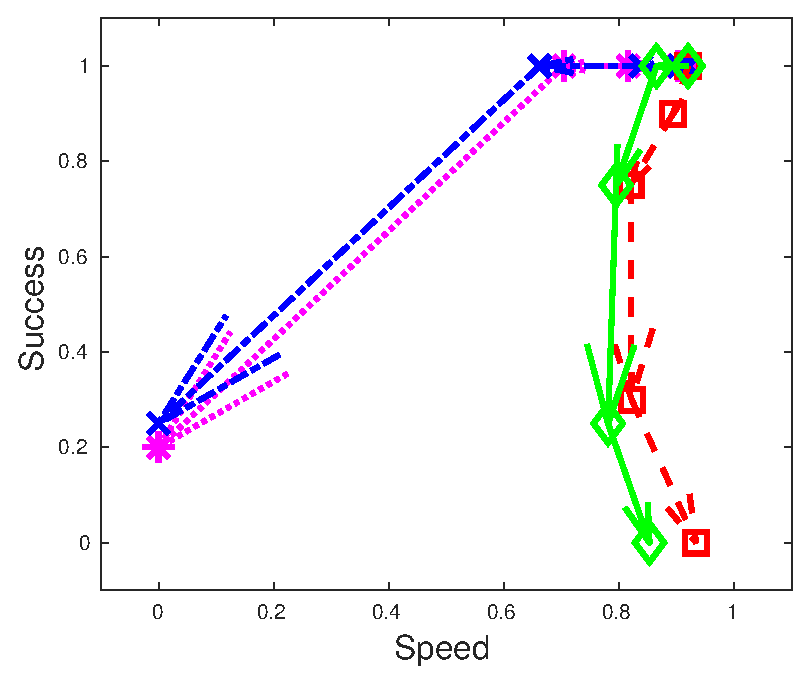
\includegraphics[width=0.3\linewidth]{simple3_speed_vs_success} \label{fig:simple3:plot_paired_metrics} }
\caption{Response of the system in the \emph{simple scenario} when varying the \emph{robot noise equally for both arms}, and activating the different planner heuristics.}
\label{fig:simple3:plots}
%
\subfloat[][Speed response.]
{\includegraphics[width=0.3\linewidth]{simple3_onearm_speed} \label{fig:simple3_onearm:speed} } \quad
%
\subfloat[][Success response.]
{\includegraphics[width=0.3\linewidth]{simple3_onearm_success} \label{fig:simple3_onearm:success} } \quad
%
\subfloat[][Speed--success trade-off.]
{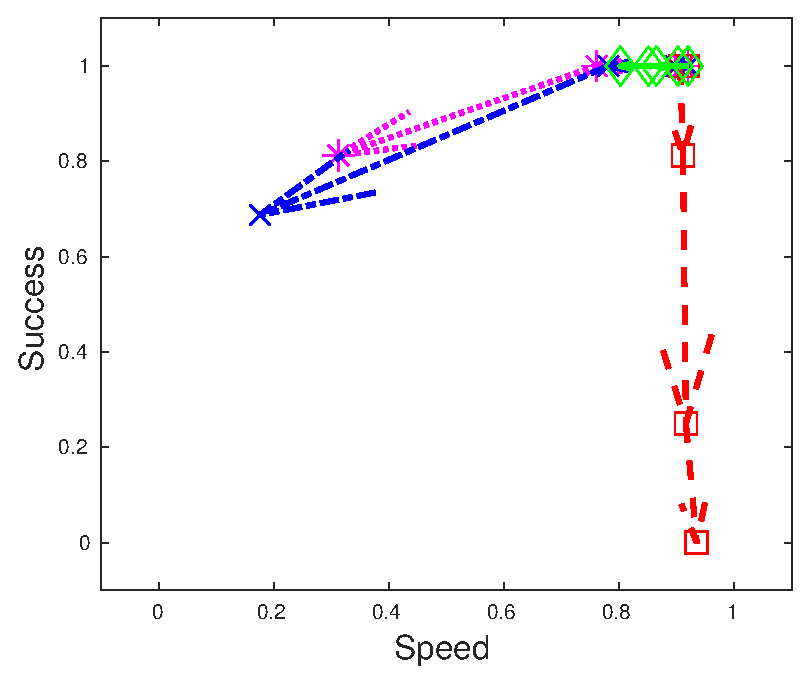
\includegraphics[width=0.3\linewidth]{simple3_onearm_speed_vs_success} \label{fig:simple3_onearm:plot_paired_metrics} }
\caption{Response of the system in the \emph{simple scenario} when varying the \emph{left arm noise}, keeping the right arm noise constant at~$0.25$, and activating the different planner heuristics.}
\label{fig:simple3_onearm:plots}
\end{figure*}

We first validate our architecture on a simple scenario which includes three objects, all within reach of the robot, as shown in Fig.~\ref{fig:simple3}.
Our system has to translate the semantic instructions to symbols, actions and goals usable by the robot.
In this case, the semantic instructions are fairly similar to the planner ones, the only significant difference being the choice of the hand~(instantiation of \fo{hand}, which can be \fo{LeftHand} or \fo{RightHand}). Depending on the simulated robot noise and on the type of planning strategy~(no heuristics; with or without Adaptability and Creativity), the behavior of the system changes as follows.

Without any heuristic~(magenta dotted line in Fig.~\ref{fig:simple3:plots}), as we introduce more noise, $\varSpeed$ decreases~(i.e., it requests a high number of $\varTotal$ actions to reach the goal), and $\varSuccess$ is constantly~$1$ (i.e., $\valTrue)$ for $\varNoise \leq 0.75$. The absence of Adaptability implies that failing actions can be executed again, up to~$t = 50$ $\varTotal$~motor actions within each episode. Despite the fact that the agent almost consistently manages to achieve the goal~($\varSuccess$ decreases only for very elevated noise), this result is disappointing from the point of view of the $\varSpeed$. Intuitively, it is not desirable that the robot try the same physical action over and over until it eventually succeeds, at the cost of considerable time wasted.
The same considerations hold for the case with the Creativity heuristic~(blue dash-dotted line in Fig.~\ref{fig:simple3:plots}), again due the absence of Adaptability~(however, the influence of Creativity would be higher if the robot noise affected only one arm instead of both arms, as we will see in the experiment of Sec.~\ref{sec:poeticon++:results:quantitative:simple_onearm}).

When we enable the Adaptability heuristic~(red dashed line in Fig.~\ref{fig:simple3:plots}), or Adaptability in conjunction with Creativity~(green solid line), as we introduce more noise, $\varSpeed$ is approximately constant~(constant $\varTotal$ attempted actions), however $\varSuccess$ decreases.
As the noise is increased, we observe some cases where the system \emph{fails} to achieve the goal~(lower \varAvgSuccess).
This is preferable to the no-heuristics and the Creativity cases, considering that $\varTotal$ is now lower, and the system can ask for external help to reach the final goal.

To summarize, when the noise is elevated we appreciate the advantage introduced by the heuristics, allowing the system to acknowledge the infeasibility of the goal when a motor action fails repeatedly, and react to it by asking for external help. This effect is more pronounced in the $\varSpeed$ metric~(see Fig.~\ref{fig:simple3:speed}), which, as defined in Eq.~\ref{eq:speed_metric}, is inversely proportional to the $\varTotal$ counter of attempted motor actions.
Fig.~\ref{fig:simple3:plot_paired_metrics} shows the trade-off between the two metrics.

\subsubsection{Simple Scenario with Unequal Arms Noise Level}
\label{sec:poeticon++:results:quantitative:simple_onearm}

In this case we start from the simple scenario and we vary the \emph{left arm noise}, keeping the right arm noise constant at~$0.25$.
Fig.~\ref{fig:simple3_onearm:plots} shows the response of the system.
The no-heuristics configuration (magenta dotted line) results in the $\varSpeed$ metric decreasing quickly, whereas $\varSuccess$ decreases only at the very end~(highest left arm noise).
When we enable the Creativity heuristic~(blue dash-dotted line) the response is similar, because Creativity alone is not effective in reacting to elevated noise in this case.

In the Adaptability case~(red dashed line), $\varSpeed$ does not decrease, but $\varSuccess$ does, and rather abruptly at that. Adaptability alone is not sufficient, in this case, because the probability of the failing action is penalized (e.g., \fo{graspWith(Ham,LeftHand)}), but the planner is not able to jump to the next sub-goal (e.g., choosing the sub-goal \fo{on(Ham,Bread)} instead of \fo{inHand(Ham,LeftHand)}).

Finally, in the Adaptability+Creativity configuration (green solid line): neither the robot $\varSpeed$ nor the $\varSuccess$ decrease much.
In particular, in Fig.~\ref{fig:simple3_onearm:plot_paired_metrics} we see that the performance always remains in the optimal region in the top-right.
Even for the most challenging left noise value, typical episodes are $\{ \varGood=4, \varTotal=9, \varSuccess=\valTrue \}$, meaning that if some left arm action fails for a few times, the planner quickly penalizes that action (Adaptability), and it is then able to jump to the next sub-goal, using the other arm (Creativity).

\subsubsection{Complex Scenario with Equal Arms Noise Level}
\label{sec:poeticon++:results:quantitative:complex}

\begin{figure*}
\subfloat[][Speed response.]
{\includegraphics[width=0.3\linewidth]{complex6_speed} \label{fig:complex6:speed} } \quad
%
\subfloat[][Success response.]
{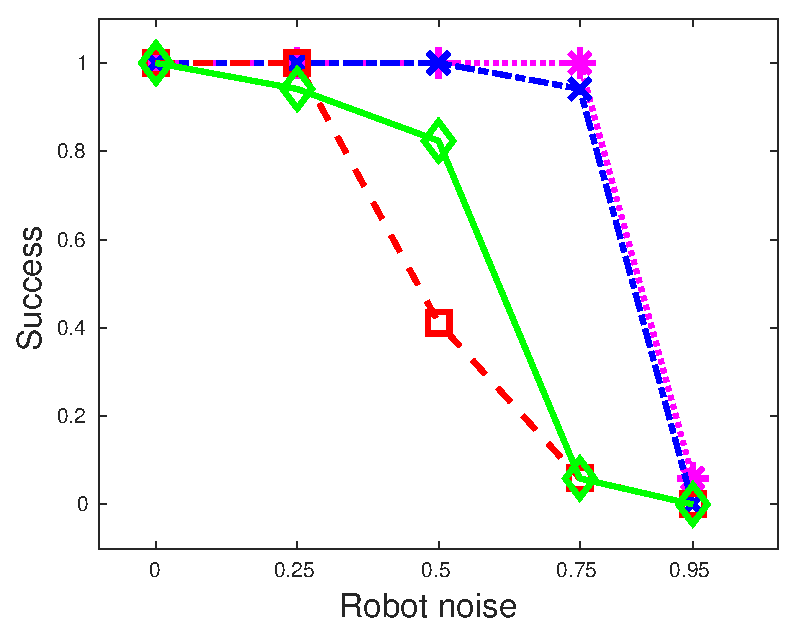
\includegraphics[width=0.3\linewidth]{complex6_success} \label{fig:complex6:success} } \quad
%
\subfloat[][Speed--success trade-off.]
{\includegraphics[width=0.3\linewidth]{complex6_speed_vs_success} \label{fig:complex6:plot_paired_metrics} }
\caption{Response of the system in the \emph{complex scenario} when varying the \emph{robot noise equally for both arms}, and activating the different planner heuristics.}
\label{fig:complex6:plots}
%
\subfloat[][Speed response.]
{\includegraphics[width=0.3\linewidth]{complex6_onearm_speed} \label{fig:complex6_onearm:speed} } \quad
%
\subfloat[][Success response.]
{\includegraphics[width=0.3\linewidth]{complex6_onearm_success} \label{fig:complex6_onearm:success} } \quad
%
\subfloat[][Speed--success trade-off.]
{\includegraphics[width=0.3\linewidth]{complex6_onearm_speed_vs_success} \label{fig:complex6_onearm:plot_paired_metrics} }
\caption{Response of the system in the \emph{complex scenario} when varying the \emph{left arm noise}, keeping the right arm noise constant at~$0.25$, and activating the different planner heuristics.}
\label{fig:complex6_onearm:plots}
\end{figure*}

We now test the system on a complex scenario which includes six objects, some of which not within the direct reach of the robot, as shown in Fig.~\ref{fig:complex6}.
This time the planner has to generate the sequence of motor commands necessary to reach faraway objects. This involves reasoning about the affordances offered by available tools, grasping a tool, and using it to draw the target object closer.
Note that, without resorting to our tool affordance model, this scenario would be always unfeasible due to the geometrical disposition of certain objects.

We first run our baseline system with no heuristics.
The results can be inspected in the magenta dotted line of Fig.~\ref{fig:complex6:plots}.
In this challenging scenario, when there is zero noise, the agent needs~$7$ motor actions to accomplish the plan.
Usually it manages to achieve it even in the presence of noise because, as in the simple scenario, these settings allow the system to retry failed actions, as long as the~$\varTotal$ action counter is at most~$t = 50$~(however, this effect gets penalized in the $\varSpeed$ metric, which decreases faster than in the simple case, as can be seen in Fig.~\ref{fig:complex6:speed} when~$\varNoise \geq 0.75$).
When we enable the Creativity heuristic~(blue dash-dotted line), the response corresponding to increasing noise is similar to the no-heuristics case.

Next, we introduce the Adaptability heuristic~(dashed red line) and then the Aptability+Creativity configuration (solid green line). We should note that, in general, the architecture manages to use the tool affordances correctly, selecting the Hook tool rather than the Stick one in order to perform a pulling action successfully~(to draw faraway objects closer to the robot workspace).
Besides, we can observe that when we introduce a considerable degree of noise~($0.5$), the $\varSuccess$ drops~(in the Creativity configuration): less than~$50\%$ of the episodes complete the plan, the majority report a failure thus requesting external help.
When the noise is even worse, $\varSuccess$ drops to zero: however, the corresponding $\varTotal$ number of attempted motor actions is kept low, minimizing the wasted time and yielding the possibility of completing the plan with further help~(e.g., with the help of the human, or with another query to the semantic reasoner given the partially-completed plan).
Enabling Adaptability and introducing noise, the system's $\varSpeed$ stays good~(a consequence of low $\varTotal$ attempted actions upon realization of failure), whereas $\varSuccess$ decreases.
The Adaptability and the Adaptability+Creativity configurations are similar, except when $\varNoise = 0.5$, where Adaptability+Creativity fares better.
Fig.~\ref{fig:complex6:plot_paired_metrics} shows the trade-off between the two metrics.

\subsubsection{Complex Scenario with Unequal Arms Noise Level}
\label{sec:poeticon++:results:quantitative:complex_onearm}

In this case we start from the complex scenario and we vary the \emph{left arm noise}, keeping the right arm noise constant at~$0.25$.
Fig.~\ref{fig:complex6_onearm:plots} shows the response of the system.
The Adaptability+Creativity configuration outperforms the other settings.
This is visible in terms of $\varSpeed$~(Fig.~\ref{fig:complex6_onearm:speed}) when the left arm noise is~$> 0.75$, and in terms of $\varSuccess$~(Fig.~\ref{fig:complex6_onearm:success}) when the left arm noise is~$> 0.5$.
For comparison, Adaptability setting has a very good $\varSpeed$, to the detriment of $\varSuccess$.

Fig.~\ref{fig:complex6_onearm:plot_paired_metrics} shows that, in this challenging experiment, the performance of our system
with heuristics
always remains in the optimal region in the top-right.
With the worst left noise value, on average the experimental episodes result in $\{ \varGood=9, \varTotal=16, \varSuccess=0.83 \}$, meaning that if some left arm action fails for a few times, the planner quickly penalizes that action (Adaptability), and it is then able to jump to the next sub-goal, using the other arm (Creativity) and being able to achieve the final goal autonomously~$83\%$ of the times.

\bigskip

With the above experiments, we have presented a quantitative evaluation which demonstrates that the combination of affordance perception with probabilistic planning and the use of planning heuristics permits to deal with high levels of noise.

\subsection{Contributions to Code Repository}
\label{sec:poeticon++:results:repo_contributions}

\begin{figure}
\includegraphics[width=0.9\textwidth]{poeticon++_software_architecture}
\caption[POETICON++ project software architecture.]{POETICON++ project software architecture. The contributions by IST are marked in red.}
\label{fig:poeticon++_sw_arch}
\end{figure}

Fig.~\ref{fig:poeticon++_sw_arch} shows the final software architecture of the POETICON++ project.
The contributions by IST are marked in red and can be further divided conceptually into:
(i)~geometrical features extractor for tool use affordances;
(ii)~world state memory;
(iii)~planning.
\myFullName{} wrote the first two components, ran the quantitative tests of the third one (see Sec.~\ref{sec:poeticon++:results:quantitative}), and integrated all the modules together.

\begin{figure}
\includegraphics[width=0.99\textwidth]{poeticon_contributors_2016-07-17}
\caption[Top contributors of the POETICON++ project repository.]{Top contributors of the POETICON++ project repository (see footnote~\footref{footnote:poeticon_repo} on p.~\pageref{footnote:poeticon_repo}). \myFullName{} is \#1 contributor in terms of number of commits.}
\label{fig:poeticon_contributors}
\end{figure}

Fig.~\ref{fig:poeticon_contributors} shows the top contributors of the POETICON++ open source project repository.
\myFullName{} is \#1 contributor in terms of number of commits, with 38.92\% of them~(\textasciitilde316 out of \textasciitilde882 total). All users had commit streaks during the periods of February--March~2015 and February--March~2016, coincident with the two last review meetings and demonstrations of the project.
If we account for actual \ac{LoC} excluding binary files, \myFullName{} had the most contributions with over~\num{65000} lines.

\section{Conclusions and Future Work}
\label{sec:poeticon++:conclusions}

This chapter presented a case study about the POETICON++ project scientific achievements, leveraging robot perception of affordances, world modeling and probabilistic planning, and supporting \hr{} collaboration behaviors.

We have described a cognitive architecture that supports action selection and complex robot manipulative task execution under challenging conditions in unstructured environments.
We combine affordance perception, world modeling and probabilistic planning to ground the semantic action plans to a robotic representation that is suitable for problem solving.
We introduce some heuristics that make the system robust to failures during task execution.

In terms of results,
(i)~we show qualitative tests on a real robot in a number of situations encountered and modeled during the POETICON++ project;
(ii)~we perform a quantitative evaluation of the system, modulating the level of noise and the use of planning heuristics.
We publicly release the code that implements our system on the iCub robot, however several software modules of our architecture can be used in other applications and platforms that include manipulative tasks.
Our release includes a simulated symbolic reasoner for validating the probabilistic planner under challenging conditions, and real robot sensorimotor data used for affordance perception.

As future work, we foresee two main aspects.
First, making the system more generic by having the robot learn the Action Rules of the domain autonomously.
Second, improving the social robot behavior aspect with further human-in-the-loop sophistication, for example by monitoring the consequences of helpful human actions in a shared \hr{} goal, and having the robot ask for confirmations~(e.g., ``did you just place this object on the table?'').
